\documentclass{article}
\usepackage{polski}
\usepackage[utf8]{inputenc}
\usepackage{amsfonts}
\usepackage{amsmath}
\usepackage{amssymb}
\usepackage{latexsym}
\usepackage{longtable}
\usepackage{natbib}
\usepackage{graphicx}
\usepackage{adjustbox}
\usepackage{algorithm2e}
\usepackage{epsfig}
\usepackage{float}


\title{Sprawozdanie z listy piątej}
\author{Karolina Bąk}
\date{Styczeń 2020}

\begin{document}
\maketitle

\section{Wstęp}
Celem tej listy zadań było stworzenie efektywnych algorytmów obliczających układ równań liniowych 
postaci $Ax = b,$ gdzie $A \in \mathbb R^{n \times n}$ jest macierzą współczynników o specyficznej strukturze, $x$ jest wektorem niewiadomych, 
a $b \in \mathbb R^n, n \geqslant 4$ jest wektorem prawych stron, bazując na eliminacji Gaussa oraz rozkładzie LU.

\subsection{Struktura macierzy A}
Macierz $A$ jest tridiagonalnie blokowa oraz rzadka. Jej strukturę można przedstawić 
w następujący sposób:
$$
A = 
\begin{pmatrix}
    A_1 & C_1 & 0 & 0 & 0 & \ldots & 0 \\
    B_2 & A_2 & C_2 & 0 & 0 & \ldots & 0 \\
    0 & B_3 & A_3 & C_3 & 0 & \ldots & 0 \\
    \vdots & \ddots & \ddots & \ddots & \ddots & \ddots & \vdots \\
    0 & \ldots & 0 & B_{v-2} & A_{v-2} & C_{v-2} & 0 \\
    0 & \ldots & 0 & 0 & B_{v-1} & A_{v-1} & C_{v-1} \\
    0 & \ldots & 0 & 0 & 0 & B_v & A_v
\end{pmatrix},
$$
gdzie $v = \frac{n}{l}$, zakładając, że $n$ jest podzielne przez $l$, $l \geqslant 2$ 
jest rozmiarem wszystkich kwadratowych macierzy wewnętrznych: $A_k, B_k$ i $C_k$. 
\newline
\newline
Macierz $A_k \in \mathbb R^{l \times l}, k = 1 \ldots v$ jest macierzą gęstą. Macierz 
$B_k \in \mathbb R^{l \times l}, k = 2 \ldots v$ jest następującej postaci:
$$
B_k = 
\begin{pmatrix}
    0 & \ldots & 0 & b_{1 l-1}^k & b_{1 l}^k \\
    0 & \ldots & 0 & b_{2 l-1}^k & b_{2 l}^k \\
    \vdots & \ldots & \vdots & \vdots & \vdots \\
    0 & \ldots & 0 & b_{l l-1}^k & b_{l l}^k 
\end{pmatrix}
$$
Natomiast $C_k \in \mathbb R^{l \times l}, k = 1 \ldots v-1$ jest macierzą diagonalną:
$$
C_k = 
\begin{pmatrix}
    c_1^k & 0 & 0 & \ldots & 0 \\
    0 & c_2^k & 0 & \ldots & 0 \\
    \vdots & \ddots & \ddots & \ddots & \vdots \\
    0 & \ldots & 0 & c_{l-1}^k & 0 \\
    0 & \ldots & 0 & 0 & c_{l}^k
\end{pmatrix}
$$
Z uwagi na specyficzną naturę macierzy A przechowuję ją w pamięci przy użyciu struktury z 
modułu SparseArrays. Dzięki temu przechowuję jedynie niezerowe elementy macierzy i oszczędzam pamięć.
Na potrzeby późniejszej analizy algorytmów przyjmuję, że dostęp do pojedynczego elementu odbywa się 
w czasie stałym, choć jest to nieprawda i będzie można zauważyć to w czasie działania algorytmów.

\section{Rozwiązywanie układu Ax = b metodą eliminacji Gauss'a}
Aby rozwiązać układ równań liniowych naturalnym wydaje się użyć eliminacji Gaussa. Klasyczny 
algorytm polega na sprowadzeniu wejściowego układu do macierzy 
trójkątnej górnej, wykorzystując do tego celu jedynie elementarne 
operacje (dodawanie, odejmowanie, mnożenie przez $l \neq 0$) na 
wierszach i kolumnach. Można także dowolnie przestawiać wiersze 
i kolumny macierzy. W efekcie otrzymujemy macierz, dzięki której, 
mając wektor prawych stron, możemy znaleźć wektor $x$ zawierający 
rozwiązania układu równań.
\newline
\newline
W celu otrzymania wynikowej macierzy trójkątnej trzeba 
wyeliminować niezerowe elementy pod przekątną macierzy. 
Stosuje się w tym celu tak zwane \textit{mnożniki}, oznaczane za pomocą 
$l_{ij}.$ W pierwszym kroku eliminowana jest niewiadoma $x_1$ z $n-1$ równań 
odejmując dla $i = 2 \ldots n$ odpowiednią krotność pierwszego równania od $i$-tego 
równania, aby wyzerować w nim współczynnik $x_1$. Zauważmy, że jest to równoznaczne z 
wyznaczeniem $x_1$ z pierwszego równania i podstawieniem do pozostałych równań. Zauważmy, 
że w celu wyzerowania elementu $a_{ik}$ należy od $i$-tego wiersza odjąć $k$-ty wiersz 
pomnożony przez współczynnik (mnożnik) $l_{ik} = \frac{a_{ik}}{a_{kk}}.$ Należy w tym momencie 
zauważyć, że algorytm nie zadziała jeśli na przekątnej wystąpi wartość 0. W tej wersji 
algorytmu można poradzić sobie z tym jedynie poprzez zamianę miejscami kolumn czy wierszy. Jednak 
nie należy zapomnieć o wprowadzeniu zmian także w wektorze prawych stron. Aby uzyskać wektor $x$, po 
zakończonej eliminacji Gaussa, trzeba wykorzystać algorytm podstawienia wstecz. 
\newline
\newline
Złożoność tego algorytmu wynosi $\mathcal{O}(n^3)$
\newline
\newline
Aby poradzić sobie z możliwymi zerami na przekątnej można lekko zmodyfikować powyższy 
algorytm. Warunek $a_{kk} \neq 0$ na ogól nie zapewnia numerycznej stabilności algorytmu. W celu 
zapobiegania problematycznym sytuacjom rozszerza się klasyczną eliminację Gaussa o wybór elementu 
głównego w kolumnie. Polega on na znalezieniu (z dokładnością do wartości bezwzględnej) największego 
elementu w kolumnie i przestawienie wierszy macierzy tak, aby wybrany element znalazł się w określonym miejscu 
na przekątnej. Można to wyrazić następującym wzorem:
$$
|a_{kk}| = |a_{s(k),k}| = max\{|a_{ik}| : i = k \ldots n \},
$$
gdzie $s(k)$ jest wektorem permutacji, w którym zapisane są przestawienia wierszy.
\newline
\newline
Poniżej przedstawię modyfikacje powyższych algorytmów dla macierzy o zadanej strukturze, których 
złożoność zbiję teoretycznie do $\mathcal{O}(n)$
\subsection{Bez wyboru elementu głównego}
Aby lepiej zobrazować modyfikację algorytmu przedstawię kawałek macierzy A:
$$
\begin{pmatrix}
    a_{11}^1 & a_{12}^1 & a_{13}^1 & a_{14}^1 & c_{11}^1 & 0 & 0 & 0 & \ldots\\
    a_{21}^1 & a_{22}^1 & a_{23}^1 & a_{24}^1 & 0 & c_{22}^1 & 0 & 0 & \ldots\\
    a_{31}^1 & a_{32}^1 & a_{33}^1 & a_{34}^1 & 0 & 0 & c_{33}^1 & 0 & \ldots\\
    a_{41}^1 & a_{42}^1 & a_{43}^1 & a_{44}^1 & 0 & 0 & 0 & c_{44}^1 & \ldots\\
    0 & 0 & b_{13}^2 & b_{14}^2 & a_{11}^2 & a_{12}^2 & a_{13}^2 & a_{14}^2 & \ldots\\
    0 & 0 & b_{23}^2 & b_{24}^2 & a_{21}^2 & a_{22}^2 & a_{23}^2 & a_{24}^2 & \ldots\\
    0 & 0 & b_{33}^2 & b_{34}^2 & a_{31}^2 & a_{32}^2 & a_{33}^2 & a_{34}^2 & \ldots\\
    0 & 0 & b_{43}^2 & b_{44}^2 & a_{41}^2 & a_{42}^2 & a_{43}^2 & a_{44}^2 & \ldots\\
    \vdots & \vdots & \vdots & \vdots & \vdots & \vdots & \vdots & \vdots & \ddots
\end{pmatrix}.
$$
Możemy zauważyć, że przy tej strukturze $A$ należy wyeliminować w każdej 
kolumnie kolejno $3,2,5,4,3,2,5,4 \ldots$ elementów. A więc ilość wyeliminowanych 
elementów w każdej kolumnie można określić wzorem:
$$
l - k \mod l \quad lub \quad 2l - k \mod l \quad dla \,(k \mod l) = (l - 1),
$$
gdzie $k$ jest numerem kolumny, a $l$ rozmiarem macierzy blokowych.
\newline
\newline
Poniżej umieszczam pseudokod obrazujący eliminację Gaussa dostosowaną 
do macierzy o zadanej strukturze.

\begin{algorithm}[H]
    \DontPrintSemicolon
    \KwIn{Macierz rzadka $A$, wektor prawych stron $b$, rozmiar macierzy $n$, rozmiar macierzy blokowych $l$} 
    \KwOut{Wektor rozwiązań $x$}
    \;
    \For{$k \gets 1$ \textbf{to} $n$} {
        $elim \gets (k \mod l) == (l - 1)\quad ? \quad k + (2l - (k \mod l)) \quad : \quad k + (l - (k \mod l))$ \\
        \For{$i \gets k+1$ \textbf{to} $elim$} {
            $mult \gets \frac{A[i,k]}{A[k,k]}$ \\
            $A[i,k] \gets 0$\\
            \For{$j \gets k+1$ \textbf{to} $min(k+l,j)$} {
                $A[i,j] \gets A[i,j] - A[k,j] * mult$\\
            }
            $b[i] \gets b[i] - b[k] * mult$
        }
    }
    $x[1:n] \gets \{0 \ldots 0\}$\\
    \For{$i \gets n$ \textbf{downto} $1$} {
        $sum \gets 0$\\
        \For{$j \gets i+1$ \textbf{to} $min(i+l,n)$} {
            $sum \gets sum + A[i,j] * x[j]$\\
        }
        $x[i] \gets \frac{b[i] - sum}{A[i,i]}$\\
    }
    \;
    \Return{$x$}
\end{algorithm}
\quad
\newline
\newline
 Można zauważyć, że główna pętla wykonuje się $n$ razy, a te wewnętrzne 
 najwyżej $l$ razy, co daje złożoność $\mathcal{O}(n*l^2)$, co daje 
 liniową złożoność, gdyż $l$ jest stałą.

\subsection{Z częściowym wyborem elementu głównego}
Przerobiony wariant eliminacji Gaussa z częściowym wyborem elementu 
głównego jest bardzo podobny do przedstawionego wyżej algorytmu z tą małą 
różnicą, że posiada też wektor permutacji, w którym są zapisane przestawienia 
elementów w kolumnach.

\begin{algorithm}[H]
    \DontPrintSemicolon
    \KwIn{Macierz rzadka $A$, wektor prawych stron $b$, rozmiar macierzy $n$, rozmiar macierzy blokowych $l$} 
    \KwOut{Wektor rozwiązań $x$}
    \;
    $perm[1:n] \gets \{1 \ldots n\}$\\
    \For{$k \gets 1$ \textbf{to} $n$} {
        $maxrow \gets k$\\
        $maxelement \gets |A[k,k]|$\\
        $elim \gets (k \mod l) == (l - 1)\quad ? \quad k + (2l - (k \mod l)) \quad : \quad k + (l - (k \mod l))$ \\
        \For{$i \gets k+1$ \textbf{to} $elim$} {
            \If{$A[k,i] \ge maxelement$}{
                $maxelement \gets |A[k,perm[i]]|$\\
                $maxrow \gets i$\\
            }
        }
        $swap(perm[k],perm[maxrow])$\\
        \For{$i \gets k+1$ \textbf{to} $elim$} {
            $mult \gets \frac{A[perm[i],k]}{A[perm[k],k]}$ \\
            $A[perm[i],k] \gets 0$\\
            \For{$j \gets k+1$ \textbf{to} $min(k+2l,j)$} {
                $A[perm[i],j] \gets A[perm[i],j] - A[perm[k],j] * mult$\\
            }
            $b[perm[i]] \gets b[perm[i]] - b[perm[k]] * mult$
        }
    }
    $x[1:n] \gets \{0 \ldots 0\}$\\
    \For{$i \gets n$ \textbf{downto} $1$} {
        $sum \gets 0$\\
        \For{$j \gets i+1$ \textbf{to} $min(i+l,n)$} {
            $sum \gets sum + A[perm[i],j] * x[j]$\\
        }
        $x[i] \gets \frac{b[perm[i]] - sum}{A[perm[i],i]}$\\
    }
    \;
    \Return{$x$}
\end{algorithm}
\quad
\newline
\newline
W przypadku eliminacji Gaussa z częściowym wyborem elementu 
głównego złożoność odrobinę wzrośnie, lecz wciąż pozostanie liniowa. 
Na wzrost złożoności ma wpływ obecność pętli, w której 
wybierany jest element główny oraz fakt, że ostatnia pętla 
w głównej pętli wykona się $2l$ razy (ponieważ ostatni niezerowy element 
można stworzyć w kolumnie $2l$, gdy eliminujemy czynniki niezerowe 
z pierwszych $l-1$ kolumn). Ostatecznie złożoność wyniesie $\mathcal{O}(n*(2l^2+l))$

\section{Rozwiązywanie układu Ax = b z uwzględnieniem rozkładu LU}
Rozkład LU jest kolejną metodą rozwiązywania układów równań 
liniowych. Jest ściśle powiązana z metodą eliminacji Gaussa. 
W tym rozkładzie wyznacza się dwie macierze trójkątne: dolną \textbf{L} 
oraz górną \textbf{U}.
\newline
\newline
Dla zadanego układu równań $Ax = b$ macierz $A$ można zapisać 
jako iloczyn macierzy \textbf{L} i \textbf{U}, gdzie:
$$
L = 
\begin{pmatrix}
    l_{11} & 0 & \ldots & 0 \\
    l_{21} & l_{22} & \ldots & 0 \\
    \vdots & \vdots & \ddots & 0 \\
    l_{n1} & l_{n2} & \ldots & l_{nn} 
\end{pmatrix}
$$

$$
U = 
\begin{pmatrix}
    u_{11} & u_{12} & \ldots & u_{1n} \\
    0 & u_{22} & \ldots & u_{2n} \\
    \vdots & \vdots & \ddots & \vdots \\
    0 & 0 & \ldots & u_{nn} 
\end{pmatrix}
$$
Wtedy początkowy układ równań przyjmuje postać $LUx = b.$ 
Jego rozwiązanie sprowadza się do rozwiązania następujących 
układów z każdą z utworzonych macierzy trójkątnych.
$$
Ux = b'
$$
$$
Lb' = b
$$
W celu zapewnienia jednoznaczności rozkładu na przekątnej 
jednej z powstałych podczas rozkładu macierzy znajdują się 
same jedynki.
\newline
\newline
Złożoność tego algorytmu jest nie większa niż $\mathcal(O)(n^2).$
\subsection{Adaptacja algorytmów}
Do optymalnego obliczania rozkładu zastosowałam przedstawione 
wcześniej algorytmy do eliminacji Gaussa, z tym, że zamiast zerować 
wartości pod przekątną umieszczam tam mnożnik użyty do 
eliminacji tego elementu. Nie liczę także wektora $x$, ani nie 
aktualizuję wektora prawych stron, gdyż te czynności wykonuję 
dopiero przy rozwiązywaniu układu przy użyciu tego rozkładu. 
Złożoność algorytmów jest taka sama, jak adaptowanych algorytmów. 
\newline
\newline
Poniżej przedstawiam pseudokody algorytmów do obliczania $Ax = b$ przy pomocy obliczonego 
wcześniej rozkładu \textbf{LU} w wariantach z wyborem elementu głównego 
oraz bez. Złożoność obu algorytmów wynosi $\mathcal{O}(2n*l)$

\subsection{Bez wyboru elementu głównego}
\begin{algorithm}[H]
    \DontPrintSemicolon
    \KwIn{Macierz rzadka $A$, wektor prawych stron $b$, rozmiar macierzy $n$, rozmiar macierzy blokowych $l$} 
    \KwOut{Wektor rozwiązań $x$}
    \;
    $b'[1:n] \gets \{0 \ldots 0\}$\\
    \For{$i \gets 1$ \textbf{to} $n$} {
        $sum \gets 0$
        \For{$j \gets max(1, l-\frac{i-1}{l})$ \textbf{to} $i-1$} {
            $sum \gets sum + A[i,j]b'[j]$ \\
        }
        $b'[i] = b[i] - sum$\\
    }
    $x[1:n] \gets \{0 \ldots 0\}$\\
    \For{$i \gets n$ \textbf{downto} $1$} {
        $sum \gets 0$\\
        \For{$j \gets i+1$ \textbf{to} $min(i+l,n)$} {
            $sum \gets sum + A[i,j] * x[j]$\\
        }
        $x[i] \gets \frac{b'[i] - sum}{A[i,i]}$\\
    }
    \;
    \Return{$x$}
\end{algorithm}
\subsection{Z częściowym wyborem elementu głównego}
\begin{algorithm}[H]
    \DontPrintSemicolon
    \KwIn{Macierz rzadka $A$, wektor permutacji $perm$, wektor prawych stron $b$, rozmiar macierzy $n$, rozmiar macierzy blokowych $l$} 
    \KwOut{Wektor rozwiązań $x$}
    \;
    $b'[1:n] \gets \{0 \ldots 0\}$\\
    \For{$i \gets 1$ \textbf{to} $n$} {
        $sum \gets 0$
        \For{$j \gets max(1, l-\frac{i-1}{l})$ \textbf{to} $i-1$} {
            $sum \gets sum + A[perm[i],j]b'[j]$ \\
        }
        $b'[i] = b[perm[i]] - sum$\\
    }
    $x[1:n] \gets \{0 \ldots 0\}$\\
    \For{$i \gets n$ \textbf{downto} $1$} {
        $sum \gets 0$\\
        \For{$j \gets i+1$ \textbf{to} $min(i+l,n)$} {
            $sum \gets sum + A[perm[i],j] * x[j]$\\
        }
        $x[i] \gets \frac{b'[i] - sum}{A[perm[i],i]}$\\
    }
    \;
    \Return{$x$}
\end{algorithm}
\section{Wyniki testów}
Dla zaimplementowanych algorytmów przeprowadziłam testy, w 
których zbadałam złożoność pamięciową oraz czasową. Do uzyskania 
danych użyłam dostępnego w Julii makra \textbf{@timed}, zwracającego 
między innymi czas działania funkcji oraz zużytą pamięć. Wyniki 
przedstawię na poniższych wykresach:

\begin{figure}[H]
    \centering
    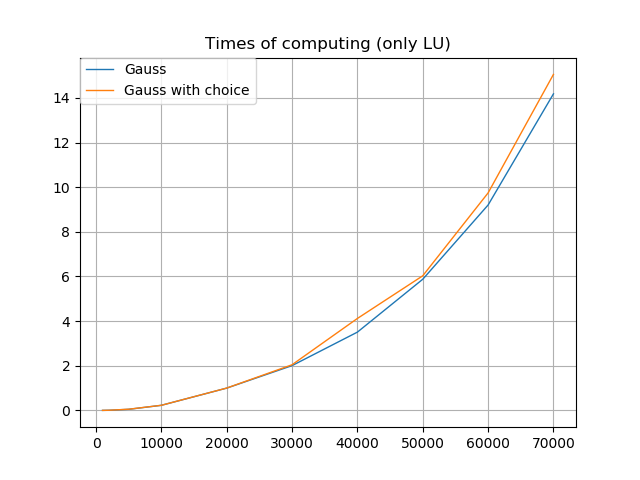
\includegraphics[width=0.45\textwidth]{times_lu.png}
    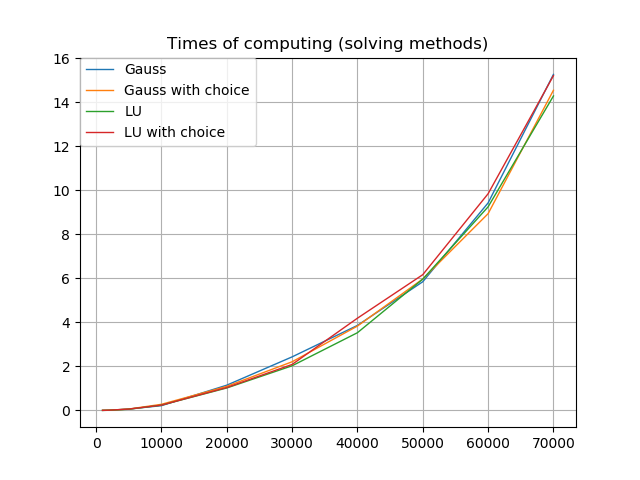
\includegraphics[width=0.45\textwidth]{times_solving.png}
    \caption{Wykresy czasu działania: 1. tylko dla rozkładu LU, 2. wszystkie metody}
\end{figure}
\begin{figure}[H]
    \centering
    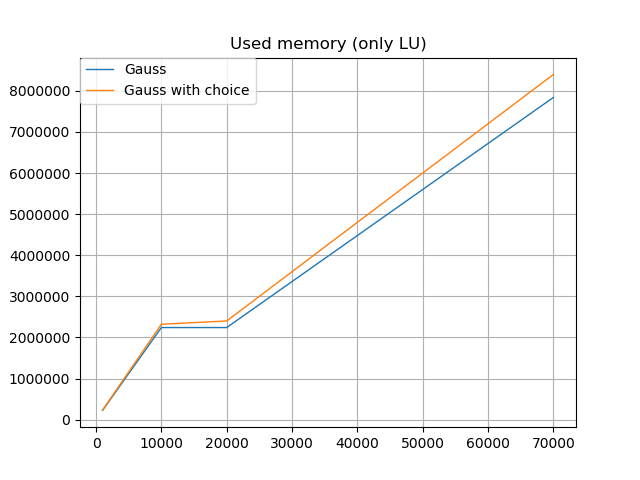
\includegraphics[width=0.45\textwidth]{memory_lu.png}
    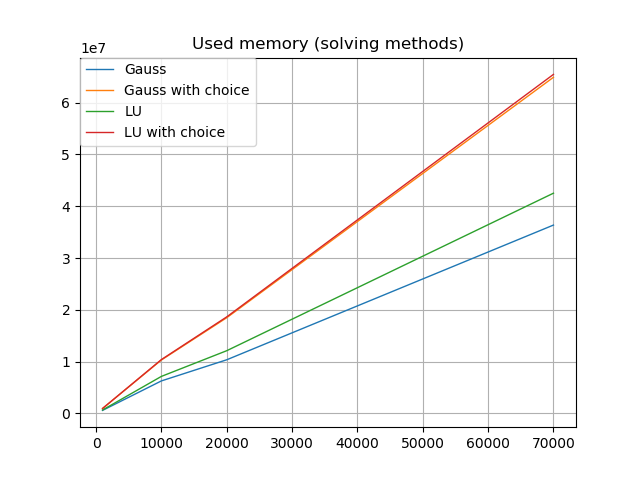
\includegraphics[width=0.45\textwidth]{memory_solving.png}
    \caption{Wykresy zużycia pamięci: 1. tylko dla rozkładu LU, 2. wszystkie metody}
\end{figure}

\section{Obserwacje}
Można zauważyć, że algorytmy używające LU oraz wyboru zużywają więcej pamięci, 
co jest zrozumiałe, gdyż w macierzy $A$ jest pamiętany także 
rozkład LU, gdzie w zwykłej eliminacji te wartości zostały wyzerowane i 
wyrzucone z pamięci, a także jest konieczność pamiętania wektora permutacji.
Z kolei rzeczywisty czas wykorzystywany przez programy jest 
funkcją kwadratową.

\section{Wnioski}
Na rzeczywisty czas wykonywania wpłynął fakt, że w SparseArrays odwoływanie 
się do elementów nie jest w czasie stałym. Jeśli jednak udało by się to 
uzyskać powyższe algorytmy działały by w czasie liniowym. Modyfikacje 
wprowadzone do klasycznych algorytmów znacznie zmniejszyły czas potrzebny na 
rozwiązywanie układów równań w tej postaci. Widać również, że 
użycie rozkładu LU jest trochę efektywniejsze czasowo (wersja bez wyboru) niż 
zwykła eliminacja Gaussa. 
\newline
\newline
Wnioskiem wynikającym z tej listy jest fakt, że czasem 
niewielkie modyfikacje klasycznych algorytmów mogą znacząco wpłynąć na 
efektywność ich działania w specyficznych przypadkach i potrafią 
prowadzić do rozwiązania skomplikowanych problemów w dość łatwy sposób.

\end{document}